\section{Timing and Hierarchical Coordination Operator between TFSM and Activity Languages}
\subsection{Overview}
In this section, we use \bcool to specify operators that capture two coordination patterns between the TFSM and Activity Language. These operators are named: \emph{startActivityWhenEnter} and \emph{AtomicActions}. The \emph{startActivityWhenEnter} operator captures a hierarchical coordination pattern. We chose the semantics in which entering a specific state of a TFSM model triggers the execution of a given fUML activity. When leaving a state, several semantic variation points may be chosen. The outgoing transitions from a state can be considered, for instance, as preemptive for the activity model (\ie firing a transition from a state to another preempts the internal activity). Alternatively, the transition can be considered as non-preemptive (\ie the states cannot be left before the associated activity finishes). In this example, we chose non-preemptive transitions.

In the \emph{AtomicActions} operator, we deal with the temporal aspects of the model coordination. The operator specifies how the time in the TFSM elapses during the execution of the activities. This coordination is also hierarchical, but in this case, only considers the timing aspects. In the TFSM language, each state machine has a \emph{localClock} used to measure the time (see Appendix~\ref{ap:languages}) while the fUML language is untimed. The local clock is a \emph{FSMClock}, which defines a \dse named \emph{ticks} whose occurrences represent a physical time increment. In the fUML language, the duration of activities can be represented as the time between the \dse \emph{startActivity} and \dse \emph{finishActivity} (see Appendix~\ref{ap:languages}). To coordinate the time, it is necessary to specify the number of \emph{ticks} of the local clock between the occurrence of the \dse \emph{startActivity} and \emph{finishActivity}. Thus, the operator enforces the execution of the ``internal'' activity to be atomic with respect to the time in the TFSM model. As a result, there is no occurrence of the \dse ticks of the corresponding local clock during the execution of the activity.

In the following, we define these operators in \bcool. In addition, we reuse the operator defined in Listing~\ref{lst:bcoolrunningexample}). Then, we use these operators to coordinate the heterogeneous model of a surveillance camera system (see Figure~\ref{fig:camerasystem}).

\subsection{Definition of the Coordination Operators}
The \emph{startActivityWhenEnter} operator (Listing~\ref{lst:bcoolStartActivityWhenEnter}) coordinates the action of entering into a state with the start of an activity so that when a state is entered, the execution of the activity is started synchronously. Then, the operator expresses that the leaving of the state follows the termination of the activity. Entering into a state is identified by the \textit{entering} \dse defined in the context of State. Instances of such \dse have to be coordinated with instances of the \textit{startActivity} \dse. Similarly, leaving a state is identified by \dse \textit{leaving} and finishing an activity is identified by \dse \textit{finishActivity}. 


The operator selects instances of \dse \emph{startActivity} and \emph{finishActivity} by using their context (Listing~\ref{lst:bcoolStartActivityWhenEnter}: line 5). The pairs selected identify the starting and finishing of an activity. Then, we select the activities that represent a state by relying on the method \emph{onEnterAction} that is defined in the context of State (see Figure~\ref{ap:languages}). It specifies the name of the activity that the state represents. To express the coordination rule, we rely on the event relation \emph{LoopFromStartToFinishNonPeemptive} (see Appendix~\ref{ap:expressionandrelations}).  As a result, the entering a state synchronously triggers the starting of an activity. Then, the activity can execute in a loop. While the activity executes, the state cannot be left. The state can be left only after the finishing of the activity. 

\begin{lstlisting}[language=bcool,
caption={Timing and Hierarchical operator between TFSM and fUML languages},
label={lst:bcoolStartActivityWhenEnter}, 
basicstyle=\scriptsize\ttfamily, backgroundcolor=\color{LGrey}, numbers=left, xleftmargin=2pt]
BCOoLSpec TFMSandActivityHierarhicalOperators
ImportLib "facilities.moccml"
ImportInterface "activitySemantics.ecl" as activity
ImportInterface "TFSM.ecl" as tfsm

Operator  StartActivityWhenEnter (activityStart : ad::startActivity , activityStop : ad::finishActivity, enterState : tfsm::entering, leaveState : tfsm::leaving)
CorrespondenceMatching: when ((activityStart.name = activityStop.name ) and (enterState.name = leaveState.name) and (activityStart.name = enterState.onEnterAction.name));
CoordinationRule: 
LoopFromStartToFinishNonPeemptive (enterState, leaveState, activityStart, activityStop)
end operator;
		
Operator AtomicActions (activityStart : ad::startActivity , activityStop : ad::finishActivity, enterState : tfsm::entering, leaveState : tfsm::leaving, timeTicks : tfsm::ticks)
CorrespondenceMatching: when ((activityStart.name = activityStop.name ) and (activityStart.name = enterState.OnEnterAction.name ) and (enterState.owningFSM.localClock = timeTicks));
CoordinationRule: 
AtomicExec (activityStart, activityStop, timeTicks)
end operator;
\end{lstlisting}
		

The \emph{AtomicActions} operator (Listing~\ref{lst:bcoolStartActivityWhenEnter}: line 11) must specify how time is consumed during the execution of the activities that are represented by states. The operator selects instances of \dse \emph{startActivity} and \emph{finishActivity} by using their context. As a result, the pairs selected identify the starting and finishing of an activity. Then, we select the activities that represent a state. To do so, we use the onEnterAction. Then, we use the selected instances of \dse entering to select instances of \dse ticks of the corresponding local clock (Listing~\ref{lst:bcoolStartActivityWhenEnter}: line 12). To express the coordination rule, we rely on the event relation \emph{AtomicExec} (see Appendix~\ref{ap:expressionandrelations}) that specifies that instances of ticks to occur only after the activity has finished its execution.
		  
The specification also contains the \emph{SyncProduct} operator that is defined in Listing~\ref{lst:bcoolrunningexample} (this is not shown in the Listing~\ref{lst:bcoolStartActivityWhenEnter}). In the following, we use this operator together with those previously defined to coordinate the heterogeneous model of a Surveillance Camera System. 


\subsection{Use of the Operators in a Surveillance Camera System}
	
\todo{to show a timing and state space exploration}
		
In this section, we develop the heterogeneous model of a surveillance camera system (see Figure~\ref{fig:camerasystem}). To model different aspects of the system, we use the TFSM and the fUML languages. Then, we use the operators developed in the previous section to coordinate the system.
	
The video surveillance system is composed of a camera and a battery control. The camera takes pictures by using either the \emph{JPEG2000} or \emph{JPG} algorithm and is powered by a battery. When the battery is low, the battery control makes the camera use the \emph{JPG} algorithm, thus reducing the quality of the picture but also the energy consumption~\cite{encodingcomparison}. When the battery is high, the JPEG2000 algorithm is used instead. In Figure~\ref{fig:camerasystem}, the activity diagrams named \emph{BatteryControl} represents the simple algorithm implemented in the battery control. At the bottom of Figure~\ref{fig:camerasystem}, the TFSM named \emph{CameraControl} represents a partial view of the camera. When the TFSM model is in state \emph{BatteryHigh}, the JPEG2000 algorithm is used (specified by the activity diagram on the right of Figure~\ref{fig:camerasystem} named \emph{doJPEG2000}). When in state \emph{BatteryLow}, the encoding algorithm is replaced by a mere JPEG algorithm represented by an activity named \emph{doJPEG} (The activity is not shown for lack of space). The transition from one state to another is done when either the \emph{BatteryIsHigh} event or the \emph{BatteryIsLow} event occurs, depending on the current state.	 
	
	\begin{figure}
		\center
		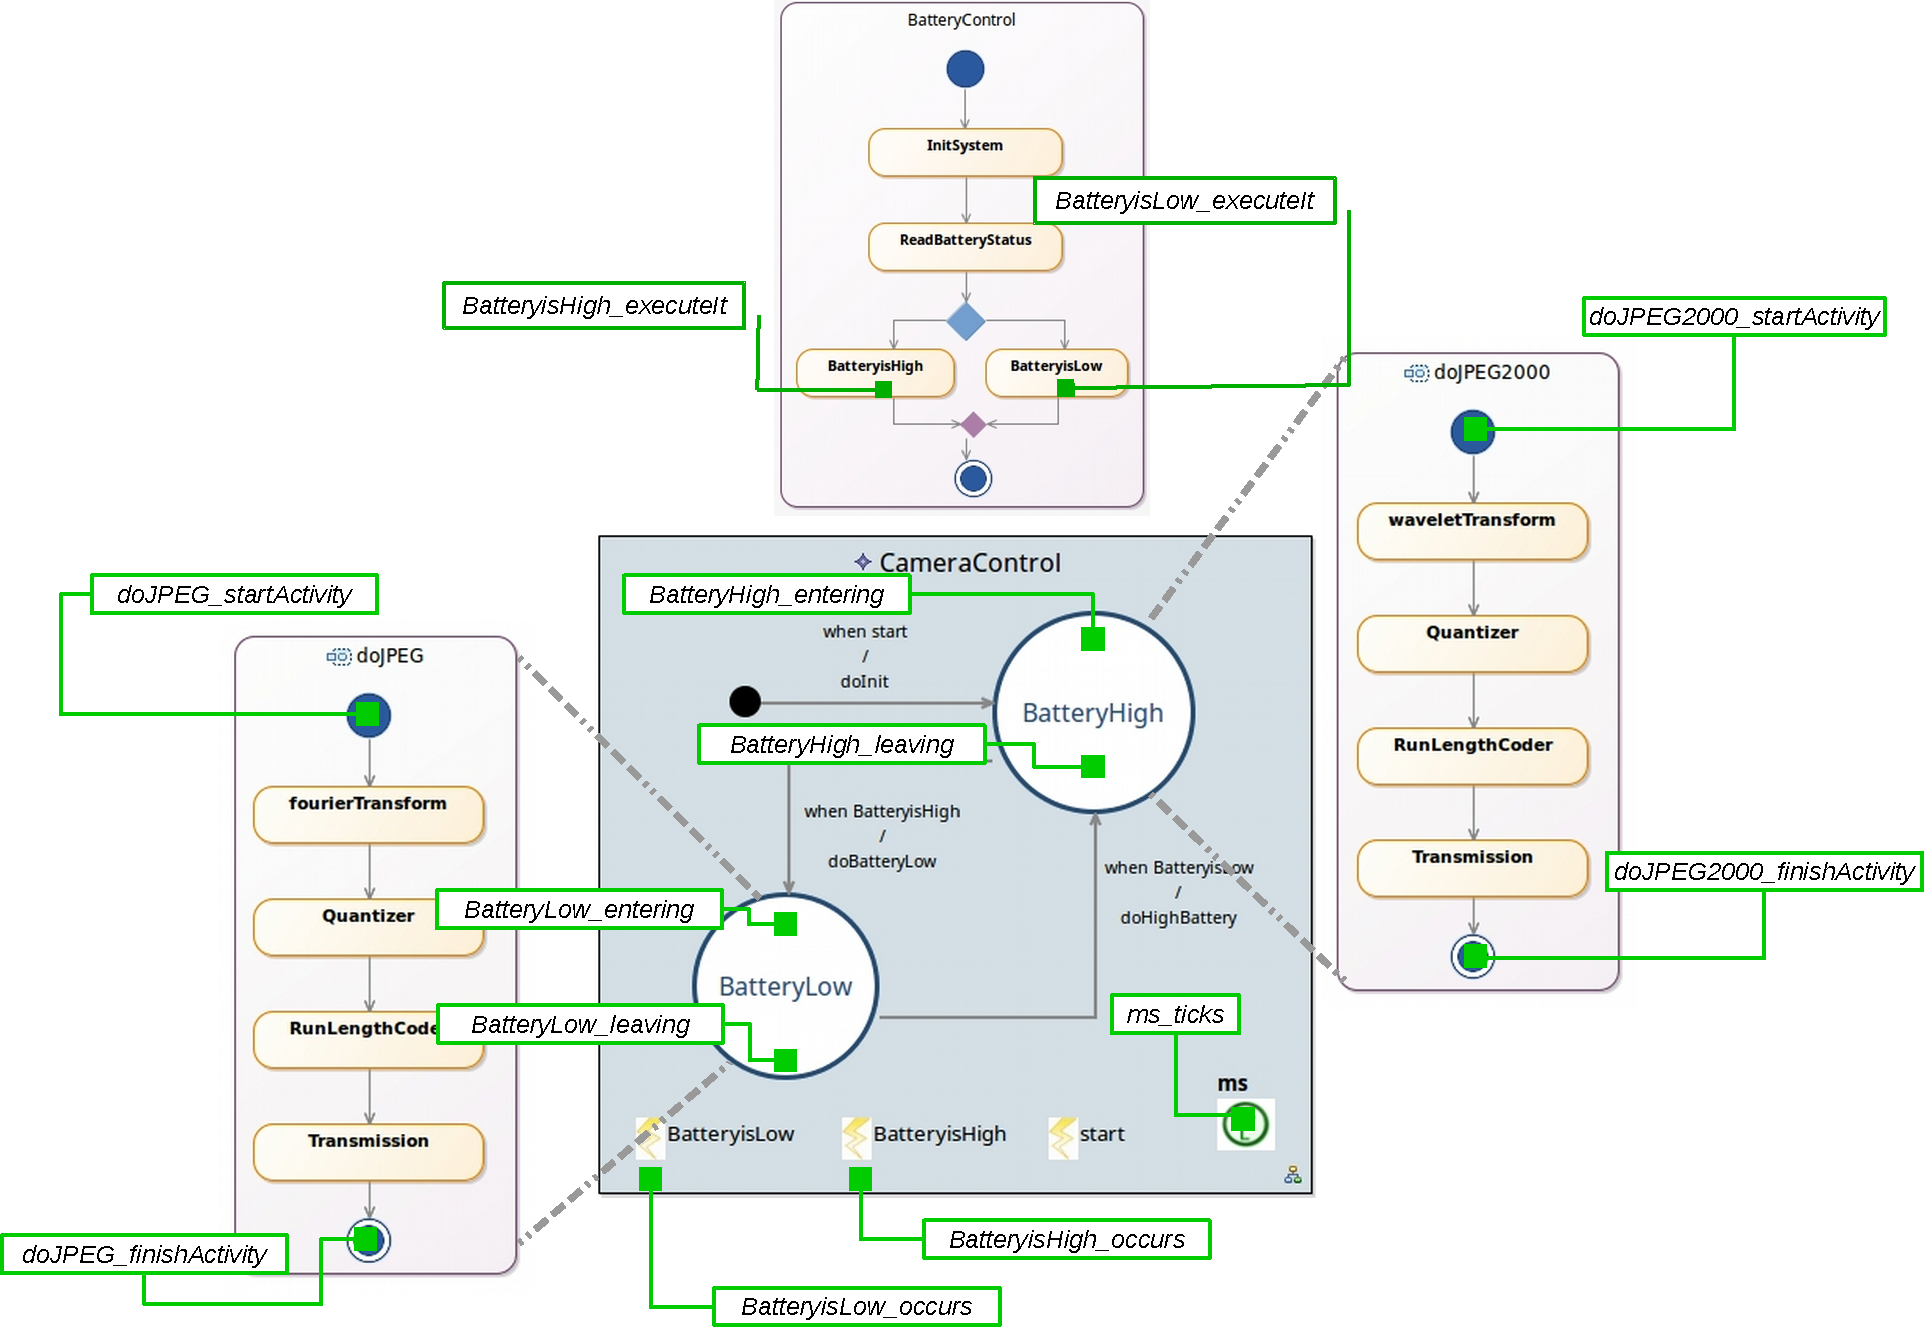
\includegraphics[width=1\columnwidth]{examples/figs/picmodels.pdf}
		\caption{Hierarchical model of a surveillance camera system and a partial representation of the behavioral interface todo: eliminate loops and add battery control}
		\label{fig:camerasystem}
	\end{figure}
	
To coordinate the models, we have to specify a timing and hierarchical coordination between the states of the TFSM CameraControl and the activities doJPEG and doJPEG2000. In addition, we have to synchronize the activity BatteryControl and the TFSM CameraControl by coordinating the corresponding Action and FSMEvent. 

\todo{
	\begin{itemize}
		\item To show the application of the operator by using the workbench.
		\item To show the application of the operators by relying on an Ant script. 
		\item To show a part of the Ant code.
	\end{itemize}
}
Applying the operators on these simple models, we generate the expected coordination specification. The coordination generated by using our approach corresponds to eight \ccsl relations.
	
By using the language workbench presented in Section~\ref{section:bcoollengbench}, the coordination specification generated for the surveillance camera system can be executed and analyzed. More precisely, we are able to execute the coordination specification by using TimeSquare, and to explore the state space. 

%For lack of space we do not show the timing output of the execution of the surveillance camera system, however, the models together with a procedure to execute and verify them can be found in the companion web site.

\subsection{Discussion}
	
\begin{itemize}
	\item \todo{Short sumarizes of the procedure followed to coordinate the models \eg \moccml, \bcool}
	\item \todo{From take-away lessons in demo}
	\item The coordination of the surveillance camera system requires the specification of eight \ccsl relations. By manually coordinating the models, this would require specifying each relation manually. The reader can notice that the number of relations increases with the number of model elements involved in the coordination. For instance, for a system with N cameras, the system designer would need to specify 8*N relations. Our proposition is to leverage this task for the system designer at the language level and then to generate all the required relations accordingly.
	
	\item We want to highlight that variations of the semantics of the resulting coordination can be done by only modifying the coordination rules of the operators. In frameworks like Ptolemy, such a variation is only supported by changing the current implementation of a \emph{director} written in Java. The same problem appears in ad-hoc translational approaches~\cite{MarcoModels2014}, where the transformation needs to be changed. Since this state of the art approach is using general-purpose transformation frameworks, this work needs a good knowledge of coordinated languages as well as a good knowledge of the transformation language itself. This is beyond the expected skills of a system designer. In our approach, we are using a language dedicated to system designer thus easing the understanding and adaptation of the \bcool specification.
\end{itemize}